In this chapter, we begin with presenting the necessary background to understand the supervised learning and data reduction methods, as well as, other ideas required to understand our research method.  We we start with the structure of CNN and the training procedure. We then discuss the modern subset selection methods that can speed up the training procedure and outline their deficiencies. Next, we review the data reduction literature and present a CNN data reduction framework - use the network pre-trained on ImageNet to extract low-dimensional features and run the data reduction methods on extracted features. Furthermore, we cover the existing trade-off framework BlinkML \cite{Park2019a} in the context of maximum-likelihood estimation machine learning algorithms and explain why it is not suitable for deep neural network. Finally, we present TAPAS \cite{Istrate2019}, which is an accuracy predictor for deep neural network without training and has several properties that make it useful to build our trade-off framework.

\section{Supervised Learning with CNN}
\label{slcnn}
CNN based supervised learning is a kind of machine learning task which learns the mapping between input visual data and output based on a set of well-labelled training samples. The visual data can be images, videos or even 3D models \cite{Song2020}. The output score after the softmax operation can be considered as the probability for a given image belongs to each class, $P(class|image, network)$. The CNN itself can be considered as a set of chained operations with trainable parameters. These parameters define the actual input-out mapping. For this reason, we use the symbol $f(x|\theta)$ to represent the output score predicted by the CNN which takes the input $x$ with a particular parameter set $\theta$. Figure \ref{Fig.CNN} gives a basic CNN structure which is designed to classify images as cats or dogs. It contains two convolutional (Conv) layers, one max pooling layer and one fully connected (FC) layer. The FC layer is actually a multi-class logistic regression model which maps the outputs of the max pooling layer to the class scores. From this perspective, we can divide the CNN structure into two parts: feature extraction part and logistic regression part. The feature extraction part performs as a blackbox which transforms the input images to points in a lower-dimensional, linearly separable space.

 \begin{figure}[H]
 \centering
 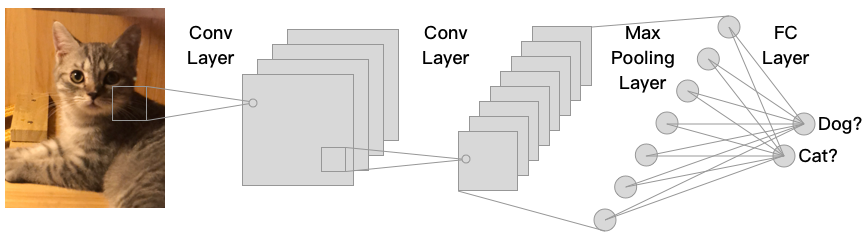
\includegraphics[width=0.8\textwidth]{src/CNN.png}
 \caption{A basic CNN structure to classify images between cats and dogs. The outputs of the penultimate layer are extracted lower-dimensional features of the input images. These features should be linearly separable to achieve a high classification accuracy}
 \label{Fig.CNN}
 \end{figure}

If we use the symbol $y$ to represent the ground truth of the input sample $x$, use $L(f(x|\theta), y)$ to represent the loss function which measures the difference between the predicted output and the ground truth label, then the training process is to find the parameter set $\theta^*$ which minimise the average loss of the whole training set as fellows:
\begin{equation}
\label{dlopt}
\theta^* = \mathop{\arg\min}_{\theta}\ \frac{1}{N}\sum^{N}_{i=1}L(f(x_i|\theta), y_i)
\end{equation}
where the symbol $N$ stands for the number of samples in the training set. This turns the training process into an optimisation problem. Different from machine learning algorithms like logistic regression and support vector machine, the equation \ref{dlopt} is non-convex thus cannot be solved analytically \cite[p.~304]{Courville2016}. A number of techniques have been developed to solve the problem with the requirement that the loss function $L(.,.)$ is continuous. The basic one to train on large dataset is called stochastic gradient descent (SGD) which updates the parameters with the partial derivatives of a randomly selected sample. At each step, the new parameter is calculated with 

\begin{equation}
	\theta_{t+1} = \theta_t - \eta
 \frac{\partial{L(f(x|\theta), y)}}{\partial{\theta_t}}
\end{equation}
and $\eta$ is the step size whose typical value is between 0.1 to 0.001. A simple variant of SGD is mini-batch gradient descent which divides the training set into disjoint subsets and averages the gradients within the subset before updating the parameters:

\begin{equation}
	\theta_{t+1} = \theta_t - \eta \frac{1}{M} \sum_{i=1}^{M}
 \frac{\partial{L(f(x_i|\theta), y_i)}}{\partial{\theta_t}}
\end{equation}
where $M$ is the batch size of the subset. For CNN, batch size $M$ is often smaller than the training set size $N$ because it takes too much memory to fit the whole dataset. Usually we use 128 or 256 as the batch size. 

\section{Mini-batch Sampling}
Since the mini-batch gradient method trains the network with a subset of samples at each step, how to select the samples becomes a problem in the deep learning literature. Instead of uniform sampling, many researchers proposed to rank the samples with importance score or classification difficulty and selects a mini-batch based on different criteria. According to \cite{Hacohen2019a}, we can divide the sampling methods into two categories: \textbf{current hypothesis method} and \textbf{targer hypothesis method}. Current hypothesis method measures the samples based on the parameter set $\theta_t$ at step $t$ while targer hypothesis method is based on the final parameter set $\theta^*$. 

\subsection{Current Hypothesis Method}
Different authors have proposed a variety of current hypothesis methods. Specifically, in self-paced learning \cite{Kumar2010, Li2017, Meng2016}, active bias learning \cite{Chang2017}, and hard example mining \cite{Shrivastava2016, Loshchilov2015}, the scores are calculated based on the sample difficulty, which is proportional to the classification score of the true class, $f(x|\theta, y)$. For importance sampling methods, the scores are calculated based on the gradient norm for each sample, $|\frac{\partial{L(f(x_i|\theta), y_i)}}{\partial{x_i}}|$. We finish this section by briefly explaining the actual implementations of these approaches.

\subsubsection{Difficulty Based Method}

Self-paced learning method tends to select easy samples which have a high classification score by injecting a pace function into the optimisation target function \ref{dlopt}:
\begin{equation}
\label{spl}
\theta^* = \mathop{\arg\min}_{\theta, v}\ \sum^{N}_{i=1} v_iL(f(x_i|\theta), y_i) + \lambda \sum^{N}_{i=1}  v_i
\end{equation}
where $v$ is the score calculated by the pace function. The pace function can be either a simple step function \cite{Kumar2010} or a more complicated dynamic function which changes with step $t$ \cite{Li2017} as long as it can assign value 0 to samples. By minimising the target function \ref{spl}, the method would zero out hard examples which have higher loss $L$ thus keep only the easy samples. This makes the trained network more robust to outliers \cite{Meng2016}. 

A potential problem of self-paced learning is that it would gradually increase the loss of hard examples \cite{Chang2017}. The possible solution is to use the active bias learning method, which is designed to select the uncertain samples whose classification score vary near the decision threshold. Chang et al. proposed and evaluated many self-paced methods and the representative one is called SGD Sampled by Threshold Closeness (SGD-STC) \cite{Chang2017}. It records the historical average classification probability $\bar{P}$ for each sample and the score is calculated with a equation that is proportional to $(1-\bar{P}) \times \bar{P}$. However, the problem is that we need extra space and computation to maintain the historical scores.

Hard example mining is yet another heuristic method aims at maximising the convergence speed by extending the self-paced learning method \cite{Shrivastava2016}. The algorithm proposed by \cite{Loshchilov2015} ranks the samples based on the latest computed classification score in descending order. At early training stages, the algorithm chooses easy samples just like self-paced learning. After a thorough exploitation process, the algorithm tends to select hard examples which have low classification scores.



\subsubsection{Importance Based Method}
Although published experiments in the cited resources above prove that difficulty based methods can surely speed up the training process and may achieve even higher accuracy, the lack of mathematical prove could lower the interests of researchers. In the contrary, importance based method raises from the profound mathematical demonstration \cite{Zhao2015} and is more reliable. Despite the elaborate derivation, the most important conclusion is that the optimal weight distribution is proportional to the per sample gradient norm.

The challenge is that computing the per sample gradient norm $|\frac{\partial{L(f(x_i|\theta), y_i)}}{\partial{x_i}}|$ is intractable. In the past few years, many researchers have adapted their approximate methods to speed up the process. The most convincing one is proposed by Katharopoulos et al. which derives an upper bound of the gradient norm \cite{Katharopoulos2018},

\begin{equation}
	|\frac{\partial{L(f(x_i|\theta), y_i)}}{\partial{x_i}}|  \leq |h(x_i)|\end{equation}
that $h(x_i)$ is the upper bound function depends on the last layer pre-activation outputs and time step $t$. With this equation, we can compute the largest sample gradient after a single forward propagation.

The benefits of current hypothesis methods is that the sample importance varies with time step thus the chosen samples at each step can reflect the current capacity of the network. However, because evaluating the whole training set is time-consuming, we often select a subset uniformly first and then select the samples within the subset. This would affect the optimal theory performance. 

\subsection{Target Hypothesis Method}
Compared with current hypothesis method, target hypothesis method selects instances based on the possible final performance of the network thus the weights of the samples are pre-defined and won't change during the training process \cite{Bengio2009}. For this reason, target hypothesis methods are more suitable to reduce the size of the dataset. To our knowledge, Curriculum Learning (CL) is the only method with these properties.

Similar with hard example mining, CL trains the network with easy samples first then adds more difficult samples into the dataset and gradually the subset would contain all the training samples. The main difference is that the difficulties of the samples are measured in advance, whether with a pre-trained network or with a linear classifier like SVM \cite{Hacohen2019a}. 

\section{Data Reduction Algorithm}
Data reduction algorithm becomes famous with the increasing of dataset size and compute time. The most common one is called Principal Components Analysis (PCA) which projects the features onto the most important few eigenvectors to capture the most variants. The famous example eigenface proves that PCA is efficient even with image dataset \cite{Paul2012}. Apart from PCA, there are other methods such as dimensionality reduction methods which reduce the size of the sample features and instance selection methods that can reduce the number of samples in the training set. We discuss some typical implementations in the next subsections.

\subsection{Dimensionality Reduction}
As discussed above, PCA is the most common method for both structured dataset and unstructured dataset. In the context of deep CNN, however, the term feature extraction is more famous as discussed in section \ref{slcnn}. Kornblith et al. evaluated the extracted features with pre-trained networks on many vision datasets and the results show that the logistic regression accuracy is linearly related to the ImageNet classification accuracy \cite{Kornblith2018}. The problem is that   



\subsection{Instance Selection}



\section{Trade-off Framework}

\section{Accuracy Predictor}